\section{Fundamentals of  Automated Planning}
\label{sec:europa}

{\footnotesize
  \begin{quote}
[Planning] \emph{is an abstract, explicit deliberation process that chooses and
organizes actions by anticipating their expected outcomes. This
deliberation aims at achieving as best as possible some prestated
objectives. Automated planning is an area of Artificial Intelligence
(AI) that studies this deliberation process computationally.} -- from
\textbf{Automated Planning Theory and Practice} by Ghallab, Nau and
Traverso \cite{ghallab04} 
\end{quote}
}

% Planning, for our purposes, can be thought of as determining all the
% small tasks that must be carried out in order to accomplish a goal.
To articulate the fundamentals of automated planning briefly and use
that to motivate the mechanisms we use in our specific form of the
technique we start with a simple example.

\begin{quotation}

  In the near future, a personal robot sets out to buy a gallon of milk
  This involves a number of tasks: obtain keys, obtain wallet,
  start car, drive to store, find and obtain milk, purchase milk, etc.
  The embedded planner has to have a ``model'' of the world in which it
  lives and has to use the task primitives in this model to structure
  the actions so it achieves its goal. Constraints control when certain
  tasks can or cannot occur. For example the robot must obtain the keys
  and wallet \emph{before} driving to the store and pick up the milk
  \emph{before} purchasing it.

\end{quotation}

For such a robot the milk buying plan at the store might look like
\comment{Figure needed}.

At the core of the \rx framework, is the deliberation engine, \eu,
which has a rich legacy from NASA missions. \eu is a versatile
Constraint-based temporal planner which continues to be deployed on a
diverse set of applications. We motivate this section with some
problem domains this planner can handle and then delve in substantial
detail.

\paragraph \textit{Constraint Satisfaction}: A canonical problem in
dealing with constraints is the $N$-Queens problem in which chess queens
must be placed on an  $N$x$N$ chessboard so no queens attack the other. Fig.
\ref{fig:nqueens-1} shows an example of a random positioning of queens
on a  $N$x$N$ chessboard. Queens in violation of the non-attack constraint
are highlighted in red.

\begin{figure} \centering
  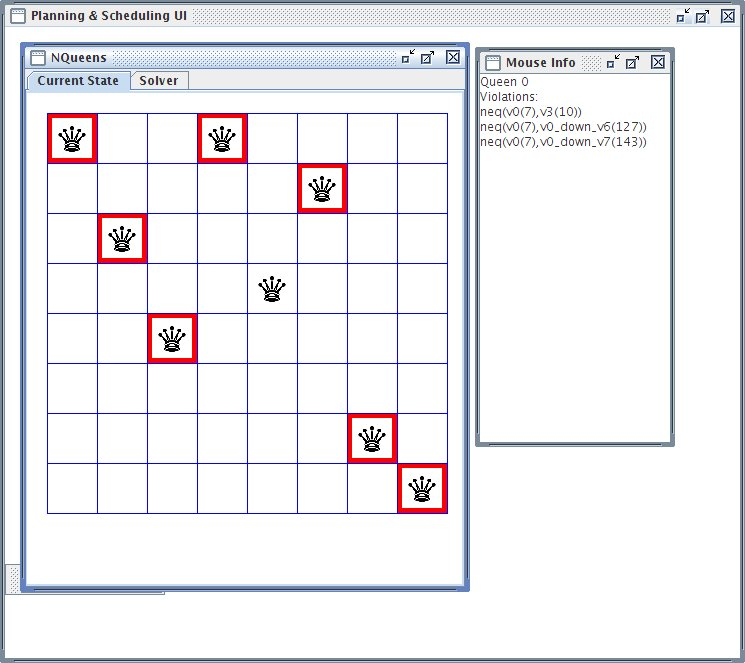
\includegraphics[scale=0.35]{figs/Example-NQueens0.jpg}
  \caption{\small N-Queens problem. Queens in violation of the
    non-attack constraint are highlighted in red.}
\label{fig:nqueens-1}
\vskip+0.1cm
\end{figure}


If we define $N$x$N$ variables Q$_{rc}$, $r \in [1,N]$, $c \in [1,N]$,
Q$_{rc} = 1$ if cell $r,c$ in the chessboard is occupied by a Queen, $0$
otherwise. Then the following constraints need to be satisfied:

\begin{equation}
 Sum(Q_{rc})= \left\{
\begin{array}{l l}
  1 & \forall r \quad \mbox{(only one Queen per row)}\\
  1 & \forall c \quad \mbox{(only one Queen per column)}\\ 
\end{array} \right.
Sum(Q_{r+i,c+i}) = 1\\
Sum(Q_{r-1,c+i}) = 1 \quad \mbox{(only one Queen on each diagonal)}\\
\end {equation} 

\comment{fix newline and numbering problem above}

The problem can be solved by finding assignments for all variables
Q$_{rc}$ that satisfy the above constraints. Fig. \ref{fig:nqueens-2} is
a solution found by \eu using that formulation and a specialized search
procedure.

\begin{figure}
\centering
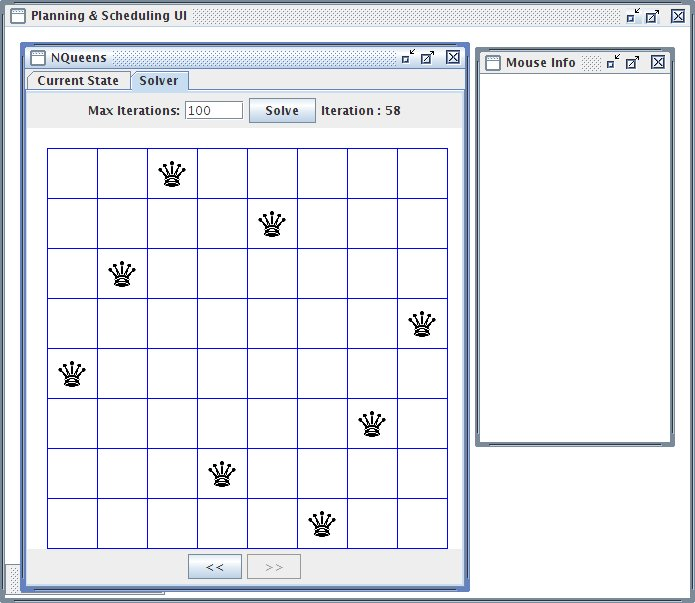
\includegraphics[scale=0.35]{figs/Example-NQueens1.jpg}
\caption{\small N-Queens solution generated by \eu}
\label{fig:nqueens-2}
\vskip+0.1cm
\end{figure}


\paragraph \textit{Scheduling}: In the Resource Constrained Project
Scheduling Problem (RCPSP) \comment{citations needed}, a project
consisting of a set of activities must be scheduled in a way that
satisfies minimum and/or maximum temporal separation constraints. The
activity schedule must also respect fixed limits on the availability of
resources required to perform each activity. In addition to satisfying
temporal and resource constraints, it is common for the user to want to
minimize makespan so that the entire project is finished as early as
possible. Fig. \ref{fig:rcpsp-1} shows an example of a a solution
provided by \eu for an RCPSP instance with 10 activities, 5 resources
and 30 temporal constraints.

\begin{figure}
\centering
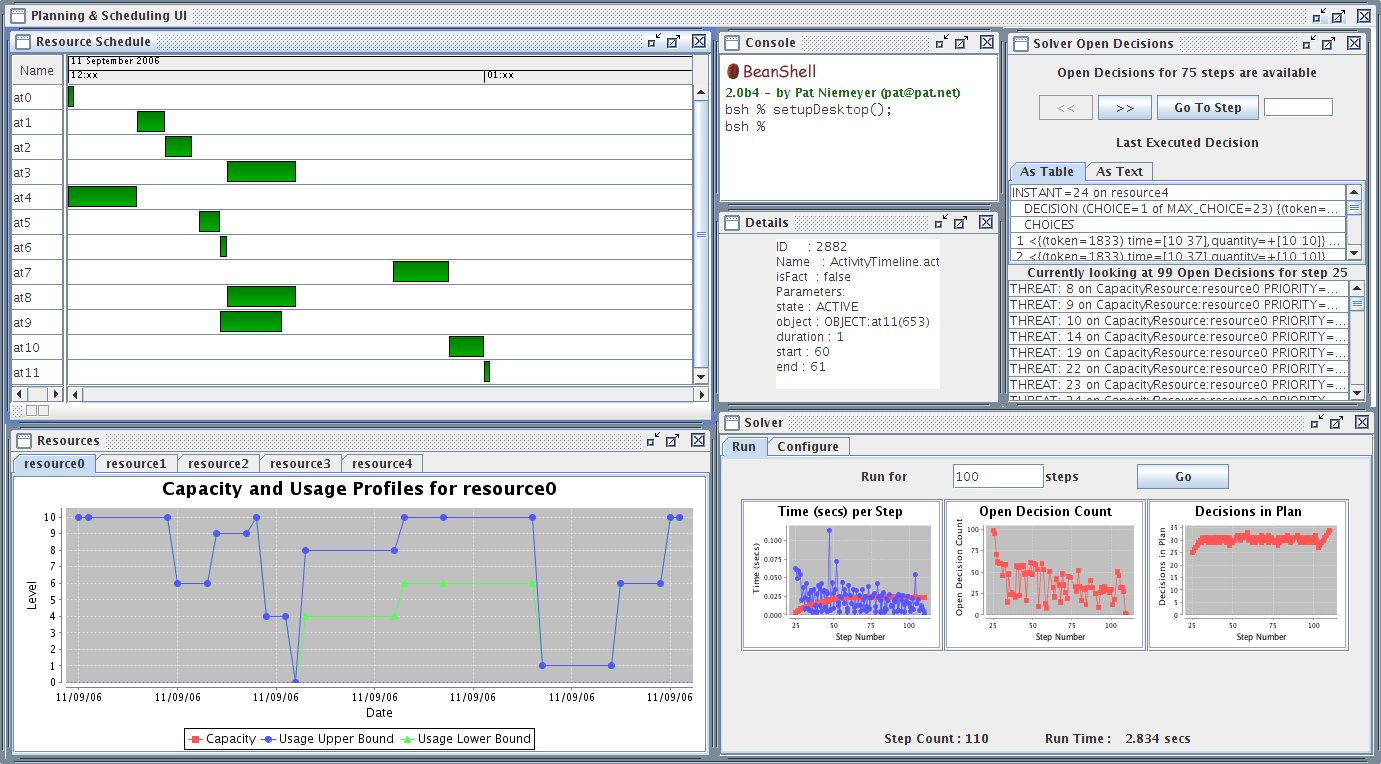
\includegraphics[scale=0.35]{figs/Example-UBO0.jpg}
\caption{\small A \eu solution to an RCPSP \comment{citation} problem.}
\label{fig:rcpsp-1}
\vskip+0.1cm
\end{figure}


\paragraph \textit{Planning}: In the Shopping Agent Problem
\cite{russelnorvig} an agent needs to purchase a set of products (milk,
drill, etc) that are available at specific locations (supermarket,
hardware store, etc), the agent is subject to temporal (must complete
tasks by specific deadlines) and resource (fuel, carrying capacity, etc)
constraints. The agent needs to figure out what actions need to be
performed to find and acquire the required items, as well as when to
perform each of those actions. Fig. \ref{fig:shopping-1} shows a
solution produced by \eu for such a problem instance.

\begin{figure}
\centering
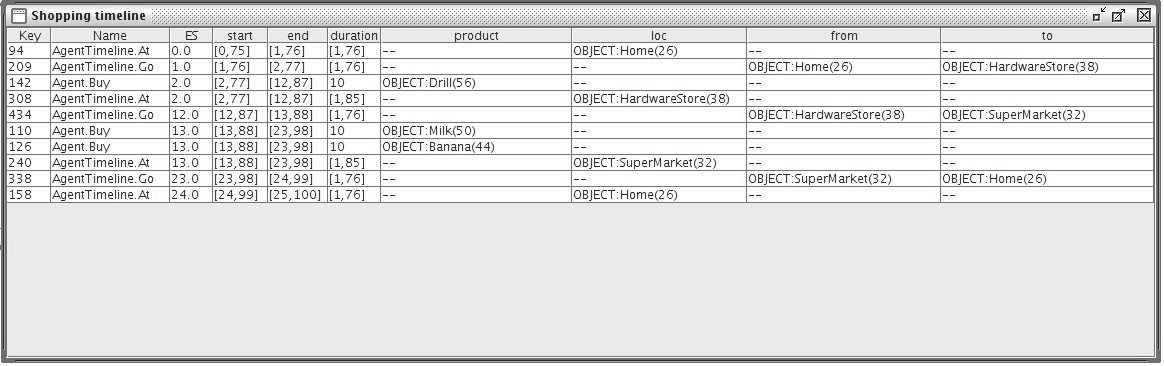
\includegraphics[scale=0.35]{figs/Example-Shopping0.jpg}
\caption{\small A \eu solution to a shopping agent problem domain where
  the agent needs to buy Bananas, Milk and a Drill.}
\label{fig:shopping-1}
\vskip+0.1cm
\end{figure}

As the examples above show, a Planning problem (actions to achieve a
goal) may embed a Scheduling problem (what resources are necessary to
achieve stated goals) and both Planning and Scheduling may embed a
Constraint Satisfaction problem. % since temporal, resource and other
% kinds of constraints must be respected in most real life problems.
The relationships between Planning, Scheduling and Constraint
Satisfaction have been examined \cite{smith00} and have lead to use of
constraint reasoning in \eu as its innermost building block. 

\subsection{Constraint Programming}
\label{sec:europa:cp}

Constraint Satisfaction Programming (also known as Constraint
Programming (CP)) is a discipline that provides a generic framework
for representing, solving and making logical inference on
constraints. A complete treatment of this discipline is given in
\cite{marriott98,apt03} and very concise introductions are provided in
\cite{bartak99,lustig01}.

A constraint programming problem consists of a set of variables $V=
{x_1,..,x_N}$, where each variable takes values from a domain
$d_1,..,d_N$; in this chapter we will deal only with discrete and
finite domains. Given a defined conjunctive set of constraints on the
variables: $C=\{c_1(x_1,..,x_N), ..., c_K(x_1,..,x_N)\}$, the
objective is to find one or more value assignments to $V$ where all
constraints are satisfied. To solve a problem, CP techniques use
logical inference to perform Constraint Propagation, which consists of
two operations:

\begin{enumerate}

\item \textbf{Bounds propagation}: To infer upper and lower variable
  bounds. For example, from the constraints $x_1 + x_2 \leq 2$ \&
  $x_i \geq 0$, we can infer $[0,2]$ bounds for $x_1$ and $x_2$

\item \textbf{Domain reduction}: To infer a valid set of values for a variable.
  For example, for  constraints allDifferent($x_1,x_2,x_3$), $x_i \geq
  0$ \& $x_i \leq 4$, if $x_1 = 1$ and $x_2 = 3$ we can infer that the
  valid domain for $x_3$ is reduced  to $\{2,4\}$

\end{enumerate}

A set of constraints and variables that describe a problem domain are
typically represented as a Constraint Network, where the variables are
nodes and constraints are arcs between the variables. Having this
network representation in mind, a pair of variables $x,y$ is said to
be arc consistent if for every value in $x$'s domain, there is a value
in $y$'s domain that is consistent with all the constraints that
connect $x$ and $y$.  A naive approach to ensuring arc consistency
consists of cycling through all the variable pairs and performing
constraint propagation until there are no variable domain changes. The
AC-3 algorithm \cite{mackworth77}, a popular implementation, improves
over the naive approach by ignoring constraints whose variables were
not affected since the last iteration.

Arc Consistency and other, more stringent consistency definitions can
be used to efficiently prove that a CP problem is
unsatisfiable. However, they generally cannot prove that a CP problem
is satisfiable and provide specific variable assignments that
constitute solutions. For that, search algorithms like global
backtracking \comment{citation needed} or local search are used; these
use consistency as an efficient way to prune the search space
\cite{cp06}. In theory, solving a CP problem is NP-Hard
\cite{ghallab04}, but often very efficient in practice using a number
of consistency and search algorithms that are well understood.

CP is usually implemented as part of a programming language and
constraints are usually represented as objects \cite{puget95}. Any
constraint that the user is able to reason about can be introduced
into the system and, as long as the constraint propagation protocols
specified by the host CP system are enforced, it will be
indistinguishable from any other "primitive'' CP constraint, such as
$\leq$ or $\geq$.

\subsection{Constraint-Based Attribute and Interval Planning}
\label{sec:europa:cp}

The most common planning formulations use a propositional
representation, where the state of the world is represented by a set
of propositions (statements that can be true or false), and operators
change the truth values of these propositions \cite{gen87}. Although
these formulations are powerful and have allowed researchers to
develop numerous contributions in automated planning, there are many
classes of problem domains that are difficult to represent using this
formalism. In particular, it is hard to represent time, resources,
mutual exclusion and concurrency using propositions \comment{citation
  needed}. While CSP representations have traditionally had an edge in
formulating and representing planning problems, 
% It is straightforward to represent and reason about all of
% those elements using a CSP representation, as a result there has been
% some work on doing automated planning while taking advantage of CSP
% (TODO: ref). Traditionally, the entire planning problem is translated
% into a CSP and then solved using traditional CSP methods, this
leading to a formulation where action choices and relationships are
represented as variables and/or constraints, there are at least two
major drawbacks:

\begin{enumerate} 

\item Given that action choices and relationships (rules) are expressed
  through variables, the domain descriptions that result from this
  approach are not intuitive and therefore difficult to understand and
  debug

\item If the structure of a planning model (actions, conditions,
  effects, dependencies at the action level) is not explicitly
  maintained by the CSP planner, the search algorithms are deprived of
  critical information to make better decisions. If that structure is
  maintained (for instance, by internally marking variables that
  represent action choice and relationships between actions), it is
  still hard to write search algorithms as any planning-specific
  insight has to be translated into the CSP representation of
  variables and constraints \comment{For example?}

\end{enumerate}

Constraint-based Planning and specifically Constraint-Based Attribute
and Interval planning (CAIP) \cite{mus94,frank2003} is intended to
close that gap. On one hand, it takes advantage of a CSP
representation; on the other it uses attributes and intervals to
maintain an explicit representation of the elements relevant to
planning. \eu is an implementation of the CAIP framework.  This makes
it easier to write algorithms that search for an reason abut
plans. The main elements of CAIP are:

\begin{enumerate}
	\item Intervals: \comment{needs to be defined}
	\item Attributes:
	\item Domain Constraints an Configuration rules:
\end{enumerate}

\comment{Explain how planning problem instances and their solutions are represented}

